% This is the root file of the thesis: thesis.tex

%%===================================
% \documentclass[12pt, oneside]{report}
\documentclass[12pt, twoside]{report}

\usepackage{url}
\usepackage[utf8]{inputenc} % This defines the font-encoding you prefer to use
\usepackage[pdftex]{graphicx}
\usepackage[bindingoffset=1cm,centering,includeheadfoot,margin=2cm]{geometry}

\usepackage[
    citestyle=numeric-comp,
    backend=biber,
    bibencoding=inputenc
    ]{biblatex}
\addbibresource{refs.bib}

\usepackage{setspace}
\linespread{1.5}
\setcounter{tocdepth}{2} 
\usepackage[colorlinks=true, pdfstartview=FitV,
linkcolor=blue, citecolor=blue, urlcolor=blue]{hyperref}
\setlength{\parindent}{0pt} % No indentation between paragraphs
\setlength{\parskip}{10pt} % Space between paragraphs

% Tables
\usepackage{ltxtable}
\usepackage{booktabs}

% Needed for code listings
\usepackage{listings}
\usepackage{color}

% Subfigure
\usepackage{subcaption}

\usepackage{floatpag} % to move floatpagenr to topright

% Fußnote
\usepackage[hang]{footmisc}
\setlength{\footnotemargin}{-0.8em}

\usepackage{csquotes}
\usepackage{afterpage} % needed for empty page after front

%%===================================
% Custom definitions
    
% Signal color
\definecolor{signalColor}{RGB}{164, 63, 114}
\newcommand\signal[1]{\textbf{\textcolor{signalColor}{#1}}}
    
% List with less space between items
\newenvironment{cList}{
\begin{itemize}
  \setlength{\itemsep}{0pt}
  \setlength{\parskip}{0pt}
  \setlength{\parsep}{0pt}
}{\end{itemize}}

% Enumeration with less space between items
\newenvironment{cEnum}{
\begin{enumerate}
  \setlength{\itemsep}{0pt}
  \setlength{\parskip}{0pt}
  \setlength{\parsep}{0pt}
}{\end{enumerate}}

% Space LoL
\let\Chapter\chapter
\def\chapter{\addtocontents{lol}{\protect\addvspace{10pt}}\Chapter}

% Code definition JSON
\definecolor{numberColor}{RGB}{24,118,129}
\newcommand\JSONnumbervaluestyle{\color{numberColor}}
\newcommand\JSONstringvaluestyle{\color{signalColor}}

\newif\ifcolonfoundonthisline

\makeatletter

\lstdefinestyle{json}{
  showstringspaces    = false,
  keywords            = {false,true},
  alsoletter          = 0123456789.,
  morestring          = [s]{"}{"},
  stringstyle         = \ifcolonfoundonthisline\JSONstringvaluestyle\fi,
  MoreSelectCharTable =%
    \lst@DefSaveDef{`:}\colon@json{\processColon@json},
  basicstyle          = \ttfamily,
  keywordstyle        = \ttfamily\bfseries
}

\lstset{
  numbers=left,
  lineskip={-1.5pt},
  captionpos=b,
  basicstyle=\footnotesize\ttfamily,
  xleftmargin=1cm,
  breaklines=true
}

\newcommand\processColon@json{%
  \colon@json%
  \ifnum\lst@mode=\lst@Pmode%
    \global\colonfoundonthislinetrue%
  \fi
}

\lst@AddToHook{Output}{%
  \ifcolonfoundonthisline%
    \ifnum\lst@mode=\lst@Pmode%
      \def\lst@thestyle{\JSONnumbervaluestyle}%
    \fi
  \fi
  \lsthk@DetectKeywords% 
}

\lst@AddToHook{EOL}%
  {\global\colonfoundonthislinefalse}

\makeatother
% End code definition JSON

% Rename listings and toc
\renewcommand{\contentsname}{Table of Contents}
\renewcommand{\lstlistlistingname}{List of Listings}

\begin{document}

%%========================================
% Frontmatter

%!TEX root = ../thesis.tex

%This is the Titlepage
%%=========================================
\thispagestyle{empty}


\includegraphics[width=\linewidth]{fig/Logo_Header}
\mbox{}\\[1pc]
\begin{center}
\huge{ \bfseries AMAZING THESIS}\\[2pc]

\Large{NAME}\\
\large{MAIL}\\[1pc]
\large{October 30, 2017}\\[2pc]

MASTER'S THESIS\\
Information Systems Engineering Chair\\
Technische Universität Berlin
\end{center}
\vfill

Examiner 1: Prof. Dr. David Bermbach
\hfill\llap{Advisor: Jonathan Hasenburg}\\
Examiner 2: SECOND EXAMINER

\afterpage{\null\thispagestyle{empty}\newpage}
 % This is the titlepage
\setcounter{page}{0}
\pagenumbering{Roman}
%!TEX root = ../thesis.tex

%This is the Preface
%%=========================================
\cleardoublepage
\section*{Sworn Affidavit}
\addcontentsline{toc}{section}{Declaration}

\begin{flushleft}
    I hereby declare that the thesis submitted is my own, unaided work, completed without any unpermitted external help. Only the sources and resources listed were used.\\
    \vspace{0.5cm}
    The independent and unaided completion of the thesis is affirmed by affidavit:\\
    \vspace{1.0cm}
    Berlin, January 1st, 1970
    \\
    \vspace{3.5cm}
    Jana Eggers
\end{flushleft}

%!TEX root = ../thesis.tex

%This is the Acknowledgment
%%=========================================
\cleardoublepage
\addcontentsline{toc}{section}{Acknowledgment}
\section*{Acknowledgment}

I would like to thank the following persons for their great support when writing my thesis at the Mobile Cloud Computing Research Group (MCC) at Technische Universität Berlin.

\begin{flushright}
INITIALS\\[1pc]
\end{flushright}

%!TEX root = ../thesis.tex

%This is the Summary
%%=========================================
\cleardoublepage
\section*{Abstract}
\addcontentsline{toc}{section}{Abstract}

FaaS is a cutting-edge new service model that has developed with the current advancement of cloud computing.
It allows software developers to deploy their applications quickly and with needed flexibility and scalability, while keeping infrastructure maintenance requirements very low.
These benefits are very desirable in edge computing, where ever changing technologies and requirements need to be implemented rapidly and the fluctuation and heterogeneity of service consumers is a considerable factor.
However, edge nodes can often provide only a fraction of the performance of cloud computing infrastructure, which makes running traditional FaaS platforms infeasible.
In this thesis, we present a new approach to FaaS that is designed from the ground up with edge computing and IoT requirements in mind.
To keep it as lightweight as possible, we use CoAP for communication and Docker to allow for isolation between tenants while re-using containers to achieve the best performance.
We also present a proof-of-concept implementation of our design, which we have benchmarked using a custom benchmarking tool and we compare our results with benchmarks of Lean OpenWhisk, another FaaS platform for the edge.
We find that our platform can outperform Lean OpenWhisk in terms of latency and throughput in all tests but that Lean OpenWhisk has higher success rates for a low number of simultaneous clients.

\newpage
\section*{Zusammenfassung}
\addcontentsline{toc}{section}{Zusammenfassung}

FaaS ist ein innovatives neues Servicemodell, das sich mit dem aktuellen Vormarsch des Cloud Computing entwickelt hat.
Softwareentwicklende können ihre Anwendungen schneller und mit der erforderlichen Flexibilität und Skalierbarkeit bereitstellen und gleichzeitig den Wartungsaufwand für die Infrastruktur sehr gering halten.
Diese Vorteile sind im Edge-Computing sehr wünschenswert, da sich ständig ändernde Technologien und Anforderungen schnell umgesetzt werden müssen und die Fluktuation und Heterogenität der Service-Consumer ein wichtiger Faktor ist.
Edge-Nodes können jedoch häufig nur einen Bruchteil der Leistung von Cloud-Computing-Infrastruktur bereitstellen, was die Ausführung herkömmlicher FaaS-Plattformen unmöglich macht.
In dieser Arbeit stellen wir einen neuen Ansatz für FaaS eine Platform vor, die von Grund auf unter Berücksichtigung von Edge-Computing- und IoT-Anforderungen entwickelt wurde.
Um den Overhead so gering wie möglich zu halten, nutzen wir CoAP als Messaging-Protokoll und Docker, um Applikationen voneinander zu isolieren, während Container wiederverwendet werden, um die bestmögliche Leistung zu erzielen.
Wir präsentieren auch eine Proof-of-Concept-Implementierung unseres Designs, die wir mit einem eigenen Benchmarking-Tool getestet haben, und vergleichen unsere Ergebnisse mit Benchmarks von Lean OpenWhisk, einer weiteren FaaS-Plattform für die Edge.
Wir stellen fest, dass unsere Plattform Lean OpenWhisk in Bezug auf Latenz und Durchsatz in allen Tests übertreffen kann, Lean OpenWhisk jedoch höhere Erfolgsraten bei einer geringen Anzahl gleichzeitiger Clients aufweist.

\tableofcontents

\clearpage
\phantomsection
\addcontentsline{toc}{section}{\listfigurename}
\listoffigures

\clearpage
\phantomsection
\addcontentsline{toc}{section}{\listtablename}
\listoftables

\clearpage
\phantomsection
\addcontentsline{toc}{section}{\lstlistlistingname}
\lstlistoflistings

%%=========================================
% Mainmatter

\cleardoublepage
\setcounter{page}{0}
\pagenumbering{arabic}
%!TEX root = ../thesis.tex

\cleardoublepage
\chapter{Introduction}
\label{cha:introduction}

This chapter gives a general introduction into the content of and the motivation for this thesis. This is done by initially outlining the motivation and problem in section \ref{sec:motivation}, defining the goal in section \ref{sec:goal}, and explaining the structure of the thesis in section \ref{sec:structure}.

%%=========================================
\section{Motivation \& Problem Description}
\label{sec:motivation}

Thus, many executives feel fear to become unconscious \cite{TheInquisitiveMind}.
Also, I want to buy \signal{smart home devices} such as the ones listed in table \ref{tab:scenario1_sensor}.

\LTXtable{\textwidth}{tab/scenario1_sensor}

%%=========================================
\section{Goal of the Thesis}
\label{sec:goal}

The goal of this thesis is to XXXXX. The contributions are:

\begin{cEnum}
    \item Analysis ...
    \item Design ...
    \item Prototypical implementation of the design.
\end{cEnum}

%%=========================================
\section{Structure of the Thesis}
\label{sec:structure}

The remainder of the thesis is structured as follows ... .

% Include more chapters as required.

%%=========================================
%Backmatter

\appendix
%!TEX root = ../thesis.tex

\cleardoublepage
\chapter{Technologies and Concepts of a Larger Context}

This appendix chapter contains definitions for technologies and concepts that are mentioned in the thesis, but are not of higher importance for it. Section \ref{sec:paxos} introduces a consensus algorithm for distributed systems.

\section{Finding Consensus in a Distributed System}
\label{sec:paxos}

The Paxos algorithm has first been described by Leslie Lamport in his work about the parliament on the island of Paxos \cite{paxos1998}. The parliament's part-time legislators had been able to maintain consistent copies of their records by following the algorithm protocol.  While the original work's main focus has not been the application in computer science, the author simplified his explanations later in \cite{paxos2001} and described how Paxos can be used to find consensus in fault-tolerant distributed systems.

Even though the Paxos algorithm cannot mitigate Byzantine failures (see appendix \ref{app:dic}), it can mitigate the effects of different processing speeds of participants and reordered, delayed, or lost messages. The only requirement is that at least half of the participants can somehow communicate.

In Paxos, four different roles exist. The \textbf{client} issues requests and waits for responses. Based on the client's request, multiple \textbf{proposer} propose a value. All these proposals are processed by the \textbf{acceptors} which will agree upon one at the end. Finally, there are the \textbf{learners} which guarantee persistence of agreed decisions and respond to client reads. The usual setup used in practice, in which every machine participating fulfills each of the roles besides the client role, is shown in figure \ref{fig:paxosSetup}.

\begin{figure}[ht]
    \centering
	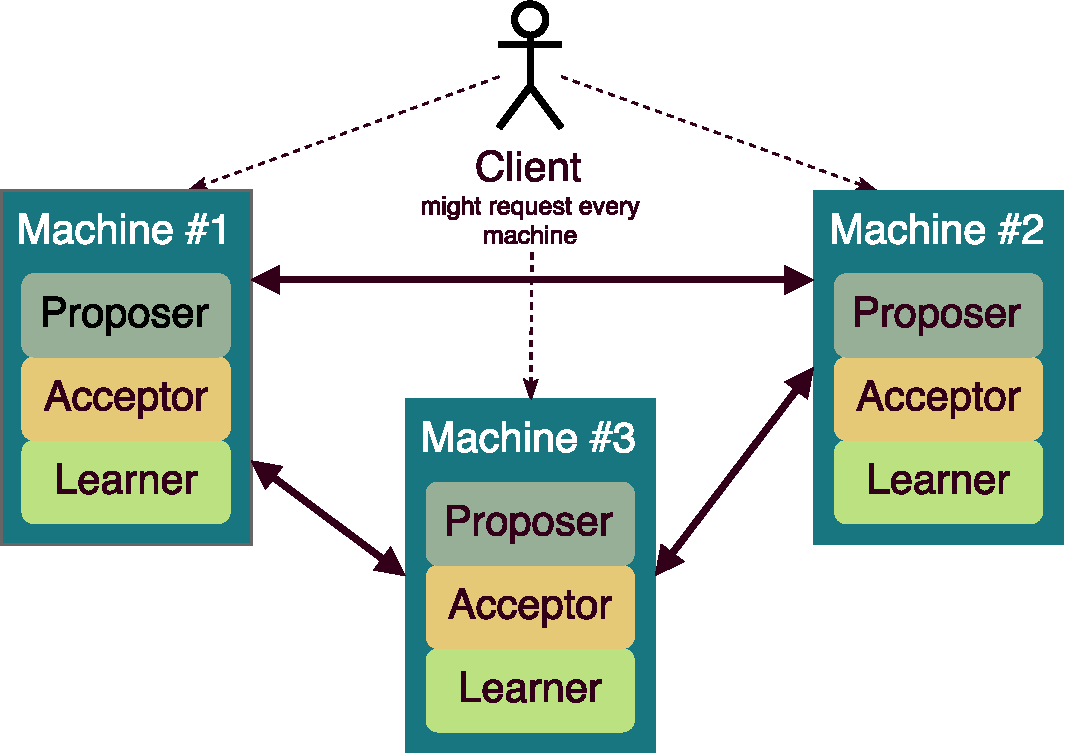
\includegraphics[width=0.8\textwidth]{fig/PaxosSetup.pdf}
	\caption{Example Setup of Three Machines Agreeing on Values Based on the Paxos Algorithm}
	\label{fig:paxosSetup}
\end{figure}

\section{Detecting Mutual Inconsistency}
\label{sec:versionVector}

Parker et al. claim that a system must ensure the mutual consistency of data copies by applying all changes made to one copy to all others correspondingly \cite{versionVektor}. Each time two copies of the same original data item have a different set of modification applied to them, they become incompatible and this conflict must be detected. However, this is not trivial, because \enquote{network partitioning can completely destroy mutual consistency in the worst case}. Nevertheless, Parker et al. state that the efficient detection of conflicts that lead to mutual inconsistency can be done by a concept they call \textit{version vectors}. They define a version vector for an item f as \enquote{a sequence of n pairs, where \textit{n} is the number of sites at which f is stored. The \textit{i}th pair ($S_i$: $v_i$) gives the index of the latest version of \textit{f} made at site $S_i$}. An example vector for an item stored at the sites A, B and D is $<$A:2, B:4, D:3$>$, which translates in a file that has been modified twice on site A, four times on site B, and thrice on site D.

A set of vectors is \enquote{compatible when one vector is at least as large as any other vector in every site component for which they have entries}. Otherwise the vectors conflict and are incompatible. E.g., the two vectors $<$A:2, B:4, D:3$>$ and $<$A:4, B:5, D:3$>$ are compatible because the second one dominates the other one. $<$A:3, B:4, D:3$>$ and $<$A:2, B:5, D:3$>$ conflict, because the first one indicates that the data item was modified one more time on node A, while the second one indicates one more modification occurred on node B. However, if we add a third vector $<$A:3, B:5, D:4$>$, no conflict exists anymore, because it dominates the two others. The consequences of an operation performed on a data item for a data item's vector is depicted in table \ref{tab:vectorOperations}.

\begin{table}[ht]
    \centering
    \begin{tabularx}{\linewidth}{@{}>{\bfseries}l@{\hspace{.5em}}X@{}}
        \toprule
        \textbf{Operation related to data item} & \textbf{Consequence for vector of data item}\\ \midrule
        Update on site $S_i$ & Increment $v_i$ by one\\
        Delete or rename on site $S_i$ & Keep vector and increment $v_i$ by one, remove data item value\\
        Reconcile version conflict & Set each $v_i$ to maximum $v_i$ from all vectors used for reconciliation. In addition, increment $v_i$ of site that initiated reconciliation by one\\
        Copy to new site & Augment vector to include new site\\
        \bottomrule
    \end{tabularx}
    \caption{Influence of Operations on a Data Item's Version Vector}
    \label{tab:vectorOperations}
\end{table}

By using version vectors, one can detect version conflicts and initiate (automatic) reconciliation. However, Parker et al. warn that two identical updates made on separate partitions will result in a conflict, even though none is present. Thus, they recommend to additionally check two data items on differences before a conflict is raised in certain applications. Furthermore, the reconciliation is most times not trivial, that's why tools such as Cassandra delegate this task to the application layer \cite{cassandra2010}.

%!TEX root = ../thesis.tex

\cleardoublepage
\chapter{Acronyms}
\begin{description}
\item[AWS] Amazon Web Services
\item[IoT] Internet of Things
\end{description}

%!TEX root = ../thesis.tex

\cleardoublepage
\chapter{Lexicon}
\label{app:dic}

\paragraph*{Byzantine failure} A malfunction of a component that leads to the distribution of wrong/conflicting information to other parts of the system is called Byzantine failure \cite{lamport1982byzantine}. The name is based on the Byzantines Generals Problem, in which three Byzantine generals need to agree on a battle plan while one or more of them might be a traitor trying to confuse the others.

%!TEX root = ../thesis.tex

\cleardoublepage
\chapter{Listings}
\label{app:listings}

This is the appendix for code, that does not need to be provided directly inside the thesis.

\section{Configuration for Node A}

\lstinputlisting[style=json, caption={Configuration for Node A}, label={lst:nodeAConfig}]{listings/nodeAConfig.js}

% Include more appendices as required.

\cleardoublepage
\addcontentsline{toc}{chapter}{Bibliography}
\defbibheading{notonline}{\chapter*{Bibliography}}
\printbibliography[heading=notonline, nottype=online]
\defbibheading{online}{\chapter*{Bibliography (Online)}}
\printbibliography[heading=online, type=online]

%%=============================================

\end{document}
